\documentclass{beamer}

% Copyright 2010 Drow Ltd.
% 
% In principle, this file can be redistributed and/or modified under
% the terms of the GNU Public License, version 2.
% 
% However, this file is supposed to be a template to be modified
% for your own needs. For this reason, if you use this file as a
% template and not specifically distribute it as part of a another
% package/program, I grant the extra permission to freely copy and
% modify this file as you see fit and even to delete this copyright
% notice. 
\mode<presentation>
{
  \usetheme[titleline=true,
            alternativetitlepage=true,
            titlepagelogo=images/Java_logo]{Torino}
  \usecolortheme{nouvelle}
  \beamertemplatenavigationsymbolsempty
}

\usepackage{helvet}
\usepackage[utf8]{inputenc}
\usepackage[english,bulgarian]{babel}
\usepackage[T2A]{fontenc}

\usepackage{listings}
\lstset{language=Java,
        captionpos=b,
        tabsize=4,
        keywordstyle=\color{blue},
        commentstyle=\color{gray},
        stringstyle=\color{green},
        numbers=left,
        breaklines=true,
        showstringspaces=false,
        basicstyle=\ttfamily,
        emph={label},
        frame=shadowbox, 
        rulesepcolor=\color{blue},
        columns=fixed}

\title{Основи програмни конструкции в Java}

\author{инж. Божидар Бацов}

\institute{Drow Ltd.}

\date{02.11.2010}

\subject{Talks}
% This is only inserted into the PDF information catalog. Can be left
% out. 

\AtBeginSection[]
{
  \begin{frame}<beamer>{Съдържание}
    \transdissolve
    \tableofcontents[currentsection,currentsubsection]
  \end{frame}
}

\begin{document}

\begin{frame}
  \titlepage
\end{frame}

\begin{frame}{Съдържание}
  \transdissolve
  \tableofcontents[pausesections]
\end{frame}

\section{Структура на Java програма}

\begin{frame}[fragile]
  \transdissolve
  \frametitle{Проста Java програма}
\begin{lstlisting}
public class SimpleClass {
  public static void main(String[] args) {
    System.out.println("Hello!");
  }
}
\end{lstlisting}
\end{frame}

\begin{frame}{Основни положения}  
  \transdissolve
  \begin{itemize}
  \item Целият код на програмата живее в класове \pause
  \item Входната точка на всяка програма е клас с main метод \pause
  \item Програмите са чувствителни към малки и големи букви \pause
  \item Имената на класовете трябва да започват с буква и да следват
    CamelCase конвенцията \pause
  \item Имената на публичните класове трябва да съвпадат с тези на
    .java сорс файлове, в които са дефинирани
  \end{itemize}
\end{frame}

\begin{frame}{Основни положения}  
  \transdissolve
  \begin{itemize}
  \item Частите(блоковете) на програмата се заграждат в \{\} \pause
  \item Програмната логика е организирана като последователност от
    твърдения \pause
  \item Твърденията се терминират с ; \pause
  \item Твърденията в една Java програма се изпълняват последователно \pause
  \item обект.метод(параметър, ...) - извикване на метод върху обект
  \end{itemize}
\end{frame}

\begin{frame}{Коментари}
  \transdissolve  
  \begin{itemize}
    \item Използват се за подобряване на четимостта на кода \pause
    \item Игнорират се от компилатора \pause
    \item Видове \pause
      \begin{itemize}
        \item C стил /* ... */ - за коментар с произволен
          размер(многоредов коментар) \pause
        \item C++ стил // - коментар до края на реда \pause
        \item javadoc /** ... */ - специален коментар
      \end{itemize}
  \end{itemize}
\end{frame}

\begin{frame}[fragile]
  \frametitle{Пример - поток на изпълнение}
  \transdissolve
  \begin{lstlisting}
public class ExecutionFlowExample1 {
  public static void main(String[] args) {
    // will be printed first
    System.out.println("Kiril");
    System.out.println("Bozhidar");
  }
}
  \end{lstlisting}
\end{frame}

\begin{frame}[fragile]
  \frametitle{Пример - поток на изпълнение}
  \transdissolve
  \begin{lstlisting}
public class ExecutionFlowExample2 {
  public static void main(String[] args) {
    // will be printed first
    System.out.println("Bozhidar");
    System.out.println("Kiril");
  }
}
  \end{lstlisting}
\end{frame}

\section{Примитивни типове данни}

\begin{frame}{Типове в Java}
  \transdissolve
  \begin{itemize}
  \item Java е силно типизиран език(strongly typed/statically typed) \pause
  \item Всяка променлива, която дефинирате трябва да има тип \pause
  \item Видове \pause
    \begin{itemize}
      \item Примитивни - числени типове, символен тип, булев тип \pause
      \item Референтни - масиви, инстанции на класове(обекти)
    \end{itemize}
  \end{itemize}
\end{frame}

\subsection{Целочислени типове}
\begin{frame}{Целочислени типове}
  \transdissolve
  \begin{itemize}
  \item byte
    \begin{itemize}
    \item размер - 1 байт
    \item граници - от -128 до 127
    \end{itemize} \pause
  \item short
    \begin{itemize}
    \item размер - 2 байта
    \item граници - от -32,768 до 32,767
    \end{itemize} \pause
  \item int
    \begin{itemize}
      \item размер - 4 байта
      \item граници - от -2,147,483,648 до
        2,147,483, 647
    \end{itemize} \pause
  \item long
    \begin{itemize}
    \item суфикс - L
    \item размер - 8 байта
    \item граници - –9,223,372,036,854,775,808 до
      9,223,372,036,854,775,807
    \end{itemize} \pause
  \end{itemize}
  Могат да се използват 8, 10 и 16тини
  бройни системи
\end{frame}

\subsection{Типове с плаваща запетая}
\begin{frame}{Типове с плаваща запетая}
  \transdissolve
  \begin{itemize}
  \item float
    \begin{itemize}
    \item суфикс - F
    \item размер - 4 байта
    \item граници - приблизително +-3.40282347E+38F
    \item значими знаци след запетаята - 6-7
    \end{itemize} \pause
    \item double
      \begin{itemize}
      \item суфикс - D
      \item размер - 15 байта
      \item граници - приблизително +-1.79769313486231570E+308
      \item значими знаци след запетаята - 15
      \end{itemize}
  \end{itemize}
\end{frame}

\subsection{Символен и булев тип}
\begin{frame}{Символен тип}
  \transdissolve
  \begin{itemize}
  \item Java има вградена поддръжка на Unicode 16 \pause
  \item char типът представя един символ в Unicode 16 кодировка \pause
  \item char константите трябва да бъдат оградени с ''(единични
    кавички) \pause
  \item Използването на char е желателно да се избягва - обикновено
    всъщност се нуждаете от низ(String) от един символ \pause
  \item Може да бъде използван и като целочислен тип без знак(unsigned
    int) с размер 2 байта
  \end{itemize}
\end{frame}

\begin{frame}{Булев тип}
  \transdissolve
  \begin{itemize}
  \item boolean - има две дискретни стойности true и false \pause
  \item 0 и null не се считат за false \pause
  \item всички логически изрази имат резултат от тип boolean \pause
  \end{itemize}
\end{frame}

\section{Променливи}
\begin{frame}{Променливи}
  \transdissolve
  \begin{itemize}
  \item Всяка променлива трябва да има
    зададен тип и име \pause
  \item Името трябва да започва с буква или \_
    и да съдържа само букви, цифри и \_ \pause
  \item Имената на променливите трябва да спазват конвенцията
    camelCase \pause
  \item Променливите трябва да бъдат инициализирани преди да бъдат използвани!
  \end{itemize}
\end{frame}

\begin{frame}[fragile]
  \frametitle{Пример}
  \transdissolve
\begin{lstlisting}
  int i; // declaration
  i = 5; // initialization
  int j = 5; // declaration + initialization
  int k, l = 13;
  long daysLeftUntilEndOfTheYear;
  char mostCommonlyUsedCharacter;
  int students;
  // ERROR - variable not initialized
  System.out.println(students);
\end{lstlisting}
\end{frame}

\begin{frame}{Свойства на променливите}
  \transdissolve
  \begin{itemize}
  \item Могат да бъдат декларирани навсякъде(преди да бъдат
    използвани) \pause
  \item Променливите имат обхват(scope) \pause
  \item Препоръчително е да бъдат дефинирани точно преди да бъде
    използвани, за да се намали обхватът им \pause
  \item На променливите(които не са маркирани като final) може да бъде
    присвоена нова стойност
  \end{itemize}
\end{frame}

\subsection{Константи}
\begin{frame}{Константи}
  \transdissolve
  \begin{itemize}
  \item За дефиниране на константи се използва ключовата дума final \pause
  \item Имената на константи се изписват по конвенцията CONSTANT\_NAME \pause
  \item Обикновено константите се дефинират на ниво клас, извън всички
    методи \pause
  \item Константите са наистина константи само за примитивни типове и
    за непроменими(immutable) референтни типове \pause
  \end{itemize}
\end{frame}

\begin{frame}[fragile]
  \frametitle{Пример - константи}
  \transdissolve
\begin{lstlisting}
public class Constants
{
   public static void main(String[] args)
   {
      final double PI = 3.14;
      double radius = 10.5;

      System.out.println("Circumference of the circle: " + 2 * PI * radius);
   }
}
\end{lstlisting}
\end{frame}

\begin{frame}[fragile]
  \frametitle{Пример - константи}
  \transdissolve
\begin{lstlisting}
public class Constants
{
   public static final double PI = 3.14;

   public static void main(String[] args)
   {
      double radius = 10.5;

      System.out.println("Circumference of the circle: " + 2 * PI * radius);
   }
}
\end{lstlisting}
\end{frame}

\section{Оператори}
\begin{frame}{Оператори}
  \transdissolve
  \begin{itemize}
  \item + - събиране \pause
  \item - - изваждане \pause
  \item * - умножение \pause
  \item / - делене – целочислено, ако и двете
    числа са цели числа, иначе с плаваща
    запетая \pause
  \item \% - остатък при делене \pause
  \item комбиниране на оператор и присвояване - +=, -=, *=, /=, \%=
  \end{itemize}
\end{frame}

\begin{frame}[fragile]
  \frametitle{Пример}
  \transdissolve
\begin{lstlisting}
int i = 5 + 8; // initialize i to 13
i = i + 5; // add 5 to i, i becomes 18
i += 5; // add 5 to i, i becomes 23
int p = i + 8; // initialize to i plus 8, i.e. 31
int q = i + p; // initialize to i plus p, i.e. 54
int t = q * 7; // initialize to q * 7, i.e. 378
\end{lstlisting}
\end{frame}

\begin{frame}{Оператори за увеличаване и намаляване с 1}
  \transdissolve
  \begin{itemize}
  \item Могат да бъдат прилагани само върху
    променливи от целочислен тип. \pause
   \item Променят стойността на променливата. \pause
   \item ++var - увеличава стойността на var с 1
    преди да бъде ползвана \pause
   \item --var - намалява стойността на var с 1,
    преди да бъде ползвана \pause
  \end{itemize}
\end{frame}

\begin{frame}[fragile]
  \frametitle{Пример}
  \transdissolve
\begin{lstlisting}
int i = 5;
++i;
System.out.println(i);   // prints 6
System.out.println(++i); // prints 7
System.out.println(i);   // prints 7
System.out.println(--i); // prints 6
System.out.println(i);   // prints 6
\end{lstlisting}
\end{frame}

\begin{frame}{Оператори за увеличаване и намаляване с 1}
  \transdissolve
  \begin{itemize}
  \item var++ - увеличава с 1 стойността на
    променливата, след като стойността е
    използвана \pause
  \item var-- - намалява с 1 стойността на
    променливата, след като стойността е
    използвана \pause
  \end{itemize}
\end{frame}

\begin{frame}[fragile]
  \frametitle{Пример}
  \transdissolve
\begin{lstlisting}
int i = 5;
i++;
System.out.println(i);   // prints 6
System.out.println(i++); // prints 6
System.out.println(i);   // prints 7
System.out.println(i--); // prints 7
System.out.println(i);   // prints 6
\end{lstlisting}
\end{frame}

\begin{frame}{Оператори за сравнение}
  \transdissolve
  Ползват се върху сравними примитивни
  типове и връщат булева стойност като резултат. \pause
  
  \begin{itemize}
  \item == - проверка за равенство
  \item != - проверка за различие
  \item $<$  - по-малко
  \item $<$= - по-малко или равно
  \item $>$  - по-голямо
  \item $>$= - по-голямо или равно
  \end{itemize}
\end{frame}

\begin{frame}{Логически оператори}
  \transdissolve
  \begin{itemize}
  \item   Логически израз се изчислява само, докато
    не е сигурна неговата стойност (short
    circuit) \pause
  \item \&\& - логическо И
  \item || - логическо ИЛИ
  \item ! - логическо отрицание
  \end{itemize}
\end{frame}

\begin{frame}{Таблица на истинност}
  \transdissolve 
  \begin{tabular}{|c|c|c|c|c|c|}
    \hline
    P & Q & P and Q & P or Q & P xor Q & not P \\
    \hline
    0 & 0 & 0 & 0 & 0 & 1 \\
    \hline
    0 & 1 & 0 & 1 & 1 & 1 \\
    \hline
    1 & 0 & 0 & 1 & 1 & 0 \\
    \hline
    1 & 1 & 1 & 1 & 0 & 0 \\
    \hline
  \end{tabular} 
\end{frame}

\begin{frame}[fragile]
  \frametitle{Пример}
  \transdissolve
\begin{lstlisting}
int x = 2;
x != 0 && 10 / x > 5; // false
!(x > 5) && x != 3; // true
x > 5 || x == 8; // false
int y = 0;
(x <5 || x > 9) && y != 0 && x + y != 0; // false
\end{lstlisting}
\end{frame}

\begin{frame}{{Автоматично преобразуване между примитивни числени типове}}
  \transdissolve
  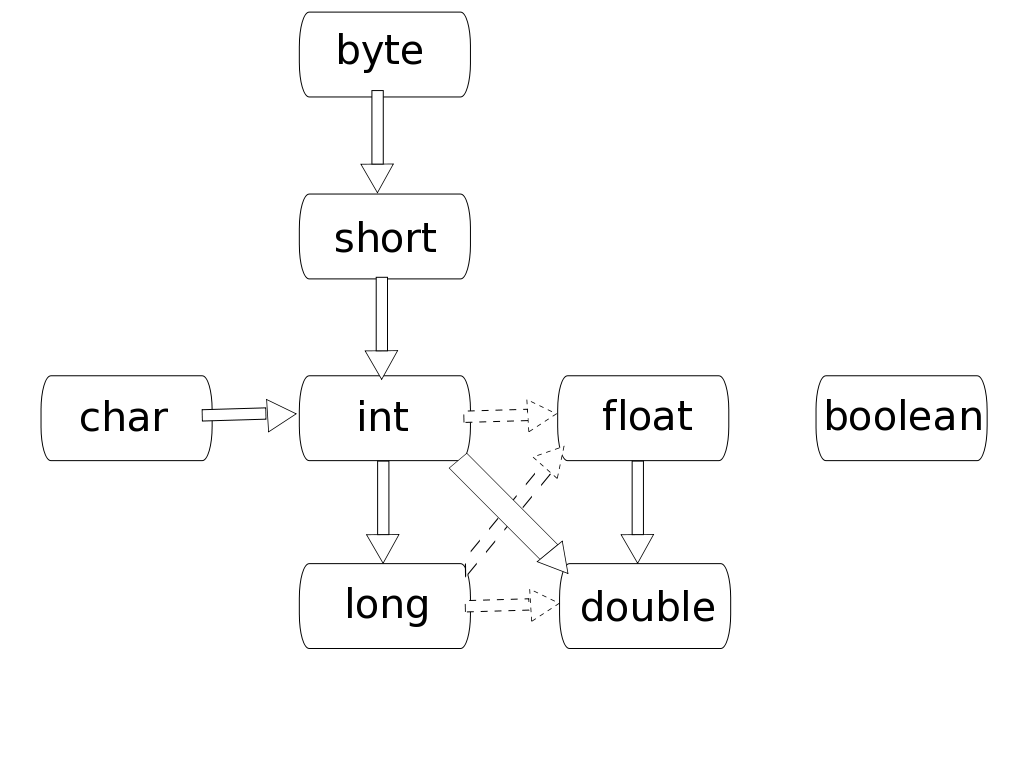
\includegraphics[height=200px, width=320px]{images/conversion.png}
\end{frame}

\begin{frame}{Автоматично преобразуване между примитивни числени типове}
  \transdissolve
  \begin{itemize}
    \item Ако единият операнд е от тип double, другият бива
      преобразуван до double. \pause
    \item В противен случай, ако единият операнд е от тип float,
      другият бива преобразуван до float. \pause
    \item В противен случай, ако единият операнд е от тип long,
      другият бива преобразуван до long. \pause
    \item В противен случай двата операнда биват преобразувани до
      int. \pause
  \end{itemize}
\end{frame}

\begin{frame}[fragile]
  \frametitle{Изрично преобразуване}
  \transdissolve
  \begin{itemize}
  \item Когато искаме преобразувания водещи
    до загуба на информация \pause
  \item ( тип-към-който-преобразуваме ) променлива
  \end{itemize}
  \begin{lstlisting}
double x = 6.79;
int i = (int) x; // i == 6
long t = 8; int q = (int) t;
  \end{lstlisting}
\end{frame}

\begin{frame}{Приоритет и асоциативност на операторите}
  \transdissolve
\small
\begin{tabular}{|c|c|}
  \hline
  Оператори & Асоциативност \\
  \hline
  [] . () (method call) & Лява \\
  \hline
  ! ~ ++ -- + (unary) (unary) () (cast) new & Дясна \\
  \hline
  * / \% & Лява \\
  \hline
  + -   & Лява \\
  \hline
  $<$ $>$$>$ $>$$>$$>$ & Лява \\
  \hline
  $<$ $<$= $>$ $>$= instanceof & Лява \\
  \hline
  == != & Лява \\
  \hline
  \& & Лява \\
  \hline
  xor & Лява \\
  \hline
  |                                      & Лява \\
  \hline
  \&\&                                   &  Лява \\
  \hline
  ||                                   &  Лява \\
  \hline
  ?:                                  &   Дясна \\
  \hline
  = += -= *= /= \%= \&= |= xor= $<$$<$= $>$$>$= $>$$>$$>$= & Дясна \\
  \hline
\end{tabular}

\end{frame}

\begin{frame}{Изброени типове}
  \transdissolve
  \begin{itemize}
  \item enum {CONS1, CONS2, CONS3...} \pause
  \item Въведени в Java 5 \pause
  \item Състоят се от краен брой константи \pause
  \item Пълноправни класове 
  \end{itemize}
\end{frame}

\section{Низове}
\begin{frame}{Низове}
  \transdissolve
  \begin{itemize}
  \item Инстанции на java.lang.String \pause
  \item Последователност от Unicode 16 символи \pause
  \item непроменими(immutable) \pause
  \item споделяни от компилатора \pause
  \end{itemize}
\end{frame}

\begin{frame}{Операции върху низове}
  \transdissolve
  \begin{itemize}
  \item Контатенация - низ1 + низ2 \pause
  \item Подниз - низ.substring(началенИндекс, бройСимволи) \pause
  \item Сравняване - низ.equals(низ2) \pause
  \item Сравняване с игнориране на размера на буквите -
    низ.equalsIgnoreCase(низ2) \pause
  \item Проверка за идентичност - низ1 == низ2
  \end{itemize}
\end{frame}

\begin{frame}[fragile]
  \frametitle{Пример - работа с низове}
  \transdissolve
\begin{lstlisting}
public class StringTest {
  public static void main(String[] args) {
    String hey = "hey hey hey ";
    String s = "some" + "string";

    System.out.println(s.substring(4));
    System.out.println(s.toUpperCase());
    System.out.println(hey + s);
  }
}  
\end{lstlisting}
\end{frame}

\begin{frame}{Работа с онлайн документация на Java}
  \transdissolve
  \begin{itemize}
  \item Интернет документация -
    http://download.oracle.com/javase/6/docs/api/ \pause
  \item Локална инсталация \pause
  \item Достъп до документацията от IDE \pause
  \end{itemize}
\end{frame}

\begin{frame}{Изграждане на низове}
  \transdissolve
  \begin{itemize}
  \item Изграждането на нови низове чрез конкатенация е уникално лоша
    идея \pause
  \item StringBuilder(въведен в Java 5) е клас специално създаден за
    тази цел \pause
  \item StringBuffer е thread-safe еквивалент на StringBuilder
  \end{itemize}
\end{frame}

\begin{frame}[fragile]
  \frametitle{Пример - изграждане на низ}
  \transdissolve
\begin{lstlisting}
public class StringBuilderTest {
  public static void main(String[] args) {
    StringBuilder sb = new StringBuilder();

    sb.append("Hello, ");
    sb.append("Java! ");
    sb.append("You rock, ");
    sb.append("Bozhidar rules!");

    System.out.println(sb.toString());
  }
}  
\end{lstlisting}
\end{frame}

\section{Вход и изход}
\begin{frame}{Конзолен вход и изход}
  \transdissolve
  \begin{itemize}
  \item Входен поток System.in \pause
  \item Прочитане на редове, низове и числа с класа Scanner \pause
  \item Извеждане на изход \pause
  \item Въвеждане на пароли с класа Console
  \end{itemize}
\end{frame}

\begin{frame}[fragile]
  \frametitle{Пример - конзолен вход и изход}
  \transdissolve
\begin{lstlisting}
public class IOTest {
  public static void main(String[] args) {
    Scanner in = new Scanner(System.in);
    System.out.print("Enter your name: ");
    String name = in.next();
    System.out.printf("Welcome back, Lord %s, Master of Java and Ruler of the Universe!%n", name);
    System.out.print("Enter a number, my liege: ");
    int number = in.nextInt();
    System.out.printf("Lord %s, the sacred number you entered is %d!%n", name, number);
  }
}  
\end{lstlisting}
\end{frame}

\begin{frame}{Форматиране на изход}
  \transdissolve
  \begin{itemize}
  \item printf - класиката си е класика \pause
    \begin{itemize}
      \item метод за форматиране на конзолен изход \pause
      \item \lstinline{System.out.printf("Hello, \%s. Next year, you'll be \%d",
        name, age);} \pause
    \end{itemize}
  \item String.format() - създаване на форматиран низ \pause
    \begin{itemize}
      \item Притежава същата семантика като printf
    \end{itemize}
  \end{itemize}
\end{frame}

\begin{frame}{Преобразувания на printf}
  \transdissolve
  \begin{tabular}{|c|c|c|}
    \hline
    Символ  & Тип                &          Пример \\
    \hline
    d & Десетично цяло число &                         159 \\
    \hline
    x & Шестнадесетнично цяло число &                 9f \\
    \hline
    o & Осмично цяло число  &                      237 \\
    \hline
    f & Число с плащава запетая &             15.9 \\
    \hline
    e & Експоненциално представяне на ЧСП &           1.59e+01 \\
    \hline
    s & Низ &                                                Hello \\
    \hline
    c & Символ &                                                 H \\
    \hline
    b &  boolean                 &                        true \\
    \hline
    tx & Дата и време &  \\
    \hline
    n & The platform-dependent line separator & \\
    \hline
  \end{tabular}

\end{frame}

\begin{frame}[fragile]
  \frametitle{Пример - форматиране на изход}
  \transdissolve
\begin{lstlisting}
public class FormatTest {
  public static void main(String[] args) {
    System.out.printf("%s has %d beers.%n", "Vasko", 20);

    System.out.printf("Today is %tc %n", new Date());

    System.out.printf("%10.2f%n", 333.444);

    System.out.println(String.format("%5d", 20));
  }
}  
\end{lstlisting}
\end{frame}

\begin{frame}{Файлов вход и изход}
  \transdissolve
  \begin{itemize}
  \item Четене на текстови файлове със java.util.Scanner \pause
  \item Запис във файл с java.io.PrintWriter \pause
  \end{itemize}
\end{frame}

\begin{frame}[fragile]
  \frametitle{Пример - файлов вход и изход}
  \transdissolve
\begin{lstlisting}
public class FileIOTest {
  public static void main(String[] args) throws FileNotFoundException {
    File someFile = new File("someFile.txt");
    PrintWriter pw = new PrintWriter(someFile);
    pw.write("One\\n");
    pw.write("Two\\n");
    pw.write("Three\\n");
    // force write to file
    pw.flush();
    Scanner in = new Scanner(someFile);
    System.out.println(in.nextLine());
    System.out.println(in.nextLine());
    System.out.println(in.nextLine());
  }
}  
\end{lstlisting}
\end{frame}

\begin{frame}{Големи числа}
  \transdissolve
  \begin{itemize}
  \item Примитивните числени типове не са подходящи за всички
    изчисления \pause
  \item java.math.BigInteger - реализира целичислен тип с неорганичен
    размер \pause
  \item java.math.BigDecimal - реализира реален тип с неограничена
    прецизност \pause
  \item Проблем на тези типове е производителността и невъзможността
    да се използват оператори с тях
  \end{itemize}
\end{frame}

\begin{frame}[fragile]
  \frametitle{Големи числа - пример}
  \transdissolve
\begin{lstlisting}
public class BigIntegerTest {
  public static void main(String[] args) {
    BigInteger someNum = BigInteger.valueOf(100);

    someNum = someNum.add(BigInteger.valueOf(50));

    // now this will be one particularly long number
    System.out.println("150 to the power of 150 is: " + someNum.pow(150));
  }
}  
\end{lstlisting}
\end{frame}

\section{Блокове}
\begin{frame}{Блокове}
  \transdissolve
  \begin{itemize}
  \item Позволява да бъдат групирани няколко
    твърдения \pause
   \item Дефиницията на блок започва с \{ и
      завършва с \} - между тях има
    твърдения \pause
   \item Имат собствен обхват \pause
   \item Могат да бъдат влагани един в друг
  \end{itemize}
\end{frame}

\begin{frame}[fragile]
  \transdissolve
  \frametitle{Блокове - пример}
\begin{lstlisting}
public static void main(String[] args) {
  int n;
  ...
  {
    int k;
    ... 
  } // k is only defined up to here
}
\end{lstlisting}
\end{frame}

\begin{frame}[fragile]
  \frametitle{Блокове - пример}
  \transdissolve
\begin{lstlisting}
public static void main(String[] args) {
  int n;
  {
    int k;
    int n; // error--can't redefine n in inner
           // block
    ...
  } 
}
\end{lstlisting}
\end{frame}

\section{Управляващи конструкции}
\subsection{Условни конструкции}

\begin{frame}{Условна конструкция if}
  \transdissolve
  \begin{itemize}
  \item Позволява условното изпълнение на код при изпълнено условие \pause
  \item if (условие) твърдение(блок от твърдения) \pause
  \item условие(condition) - логически израз \pause
  \item твърдение - действие, което да бъде
    изпълнено, ако условието е вярно
  \end{itemize}
\end{frame}

\begin{frame}[fragile]
  \frametitle{if - пример}
  \transdissolve
\begin{lstlisting}
if (performance > 5) {
  salary+=500;
  bonus = 100;
}
\end{lstlisting}
\end{frame}

\begin{frame}{Условна конструкция if-else}
  \transdissolve
  \begin{itemize}
  \item if (condition) statement1 else statement2 \pause
  \item condition - логически израз \pause
  \item statement1 - твърдение, което да бъде
      изпълнено, ако условието е вярно \pause
  \item statement2 - твърдение, което да бъде
    изпълнено, ако условието е невярно \pause
  \end{itemize}
\end{frame}

\begin{frame}[fragile]
  \frametitle{if-else - пример}
  \transdissolve
\begin{lstlisting}
if (performance > 5) {
    salary += 500;
    bonus = 100;
} else {
    bonus = 0;
}
\end{lstlisting}
\end{frame}

\begin{frame}[fragile]
  \frametitle{if-else-if-else}
  \transdissolve
\begin{lstlisting}
if (performance > 5) {
  salary += 500;
  bonus = 100;
} else if (performance > 2) {
  salary += 100;
  bonus = 0;
} else { 
  // you're fired
  salary = 0; 
  bonus = 0; 
}
\end{lstlisting}
\end{frame}

\begin{frame}[fragile]
  \frametitle{Множествен избор със switch}
  \transdissolve
  \begin{itemize}
  \item Множествен избор - switch \pause
  \item може да се
    използва с byte, short, char, int \pause
  \end{itemize}
  \begin{lstlisting}
switch (variable) {
  case VALUE : statements;
  case VALUE : statements;
  default : statements;
}
  \end{lstlisting}
\end{frame}

\begin{frame}[fragile]
  \transdissolve
  \frametitle{switch - пример}
\begin{lstlisting}
int month = 8;
switch (month) {
case 1: 
  System.out.println("January"); break;
  ...
case 12:
  System.out.println("December"); break;
default: 
  System.out.println("Invalid month."); break;
}
\end{lstlisting}
\end{frame}

\begin{frame}[fragile]
  \frametitle{switch - пример}
  \transdissolve
\begin{lstlisting}
int startFrom = 6;
switch (month) {
case 1: System.out.println(1);
...
case 6: System.out.println(6);
case 10: System.out.println(10); break;
default: System.out.println("Invalid number."); break;
}
\end{lstlisting}
\end{frame}

\subsection{Цикли}

\begin{frame}{Цикъл while}
  \transdissolve
  \begin{itemize}
  \item Синтаксис - while (condition) \{statement(s);\} \pause
    \begin{itemize}
      \item условие(condition) определя дали ще изпълни тялото на
        цикъла \pause
      \item тялото на цикъла се състои от едно или повече твърдения \pause
    \end{itemize}

  \item Семантика - цикълът while може и ДА НЕ СЕ изпълни нито веднъж \pause
  \item Поток на изпълнение - след изпълнение на тялото контрола се
    прехвърля в условието на цикъла
  \end{itemize}
\end{frame}

\begin{frame}[fragile]
  \frametitle{Цикъл while - пример}
  \transdissolve
\begin{lstlisting}
int money = 20;
int beersDrank = 0;
while (money > 5) {
    money -= 3; // buy beer
    beersDrank++;
}
System.out.print("We've drunk " +  beersDrank + " beers.");
\end{lstlisting}
\end{frame}

\begin{frame}{Цикъл do-while}
  \transdissolve
  \begin{itemize}
  \item Синтаксис - do \{statements\} while (condition) \pause
  \item Семантика - цикълът do-while се изпълнява винаги поне веднъж
  \end{itemize}
\end{frame}

\begin{frame}[fragile]
  \frametitle{Цикъл do-while - пример}
  \transdissolve
\begin{lstlisting}
int count = 1;
do {
    System.out.println("Count is: " + count);
    count++;
} while (count <= 11);
\end{lstlisting}
\end{frame}

\begin{frame}{Цикъл for}
  \transdissolve
  \begin{itemize}
  \item for ( initialization; condition; update )  {statement} \pause
  \item initialization инициализираме променливи \pause
  \item condition логически израз \pause
  \item update - изпълнява се, докато
    условието е вярно, преди statement \pause
  \item statement - изпълнява се, докато
    условието е вярно, след update
  \end{itemize}
\end{frame}

\begin{frame}[fragile]
  \frametitle{Цикъл for - пример}
  \transdissolve
\begin{lstlisting}
for (int i = 1; i <= 10; i++) {
  System.out.println(i);
}
// i no longer defined
int i;
for (i = 1; i <= 10; i++) {
  System.out.println(i);
}
// i still defined
\end{lstlisting}
\end{frame}

\begin{frame}[fragile]
  \frametitle{Прекратяване на цикъл преждевременно}
  \transdissolve
  \transdissolve
  \begin{block}{break}
    break прекратява текущия цикъл(или блок). Може
    да се ползва в for, while, do-while и
    switch.
  \end{block}
\begin{lstlisting}
int i;
for (i = startNumber; i < startNumber + 5; i++) {
  if (i % 5 == 0) break; 
}
System.out.println("closest number : " + i);
\end{lstlisting}
\end{frame}

\begin{frame}[fragile]
  \frametitle{Преминаване към следващата итерация}
  \transdissolve
  \begin{block}{continue}
    преминаване към следваща
    итерация в цикъл. Може да се
    използва в for, while, do-while цикли
  \end{block}
\begin{lstlisting}
int numbersNotDivideableByThree = 0;
for (int i = startValue; i < 1000; i++) {
     if (i % 3 == 0) continue;
     numbersNotDivideableByThree++; 
}
\end{lstlisting}
\end{frame}

\section{Масиви}

\begin{frame}{Масив}
  \transdissolve
  \begin{itemize}
    \item съдържа набор от елементи от един тип \pause
    \item достъпът до елементи се осъществява по индекс(позиция) \pause
    \item индексите започват от 0(Нула) \pause
  \end{itemize}
  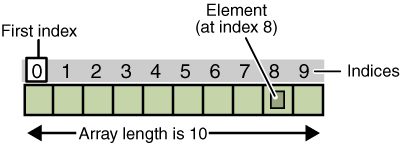
\includegraphics[width=300px,height=100px]{images/array.png}
\end{frame}

\begin{frame}{Свойства на масивите}
  \transdissolve
  \begin{itemize}
  \item arr.length ни дава дължината на един масив \pause
  \item има предефинирана дължина и тя не може да бъде
    променена \pause
  \item може да има повече от едно измерение
  \end{itemize}
\end{frame}


\begin{frame}{Създаване и инициализиране на масиви}
  \transdissolve
  \begin{itemize}
  \item Декларация
    \begin{itemize}
      \item type[] arrVariable;
      \item type arrVariable[];
    \end{itemize}
  \item Създаване на масив
    \begin{itemize}
      \item new type[size]
    \end{itemize}
  \item Инициализация със списък от стойности
  \item Анонимен масив
  \end{itemize}
\end{frame}

\begin{frame}[fragile]
  \frametitle{Масив - декларация, създаване и инициализация}
  \transdissolve
\begin{lstlisting}[basicstyle=\tiny]
class ArrayDemo {
  public static void main(String[] args) {
    int[] anArray; // declares an array of integers             

    anArray = new int[10]; // allocates memory for 10 integers
           
    anArray[0] = 100; // initialize first element
    anArray[1] = 200; // initialize second element
    anArray[2] = 300; // etc.

    System.out.println("Element at index 0: " + anArray[0]);
    System.out.println("Element at index 1: " + anArray[1]);
    System.out.println("Element at index 2: " + anArray[2]);
  }
} 
\end{lstlisting}
\end{frame}

\begin{frame}[fragile]
  \frametitle{Масив - пример}
  \transdissolve
\begin{lstlisting}
String[] names = { "Pesho", "Gosho", "Ivan" };

for (int i=0; i < names.length; i++) {
  System.out.println("Name : " + names[i]);
}
\end{lstlisting}
\end{frame}

\begin{frame}[fragile]
  \frametitle{Масив - пример}
  \transdissolve
\begin{lstlisting}
int[] numbers = { 1, 8, 10, 33 };
long sum = 0;

for (int i = 0; i < numbers.length; i++) {
  sum += numbers[i];
}

System.out.println("Sum : " + sum);
\end{lstlisting}
\end{frame}

\begin{frame}{Цикъл for-each}
  \transdissolve
  \begin{itemize}
  \item For-each цикъл
    \item for (array-type variable : array) statement

    \item Array-type – тип на променливата
    –variable, трябва да съвпада с типа на
    елементите в масива
    \item Variable – променлива, съдържаща
    текущия елемент от масива
    \item Array – масив, от който да бъдат
    взимани елементи

  \end{itemize}
\end{frame}

\begin{frame}[fragile]
  \frametitle{Цикъл for-each - пример}
  \transdissolve
\begin{lstlisting}
public class ForEachLoopTest {
  public static void main(String[] args) {
    for (String name : new String[]{"Bozhidar", "Ivan", "Ana", "Iva", "Andrey"}) {
      System.out.printf("%s is a really cool name!%n", name);
    }
  }
}  
\end{lstlisting}
\end{frame}

\begin{frame}{Основни операции с масиви}
  \transdissolve
  \begin{itemize}
    \item Отпечатване
      \begin{itemize}
        \item С цикъл
        \item Arrays.toString(array)
      \end{itemize}
    \item Копиране
      \item Присвояването не работи - така няколко променливи споделят
        един масив
      \item System.arraycopy()
      \item Arrays.copyOf()
    \item Сортиране
  \end{itemize}
\end{frame}

\begin{frame}{Параметри от командния ред}
  \transdissolve
  \begin{itemize}
  \item Предават се под формата на масив от низове на метода main()
  \item Разделят се с интервали или табулации
  \item За разработка на конзолно приложение с гъвкави аргументи ще ви
    трябва външна библиотека като JArgs, JOpts и Commons CLI
  \end{itemize}
\end{frame}

\begin{frame}{Многоизмерни масиви}
  \transdissolve
  \begin{itemize}
  \item Позволяват представянето на комплексни данни в масив
  \item Java не поддържа истински многоизмерни масиви
  \item Декларация и създаване на много измерен масив
    \begin{itemize}
      \item type[][] someArr = new type[3][3];
    \end{itemize}
  \end{itemize}
\end{frame}

\begin{frame}{Упражнение}
  \transdissolve  
  \begin{enumerate}
    \item Намерете сумата на първите хиляда естествени числа. \pause
    \item Намерете сумата на всички естествени числа, които са
      по-малки от хиляда и се делят на 3 и 5 без остатък. \pause
    \item Намерете сумата от цифрите на 100!(факториел). \pause
    \item Намерете броят на необходимите букви за изписването на
      всички числа между 1 и 1000(включително) на английски език.
  \end{enumerate}

\end{frame}

\section*{Заключение}

\begin{frame}{Заключение}
  \transdissolve
  % Keep the summary *very short*.
  \begin{itemize}
  \item
    Примитивните типове от данни са в основата на \alert{всички} Java приложения.
  \item
    Управляващите конструкции ви позволяват да манипулирате потокът на
    изпълнение на една Java програма.
  \item
    Масивите предоставят начин за групиране на свързани елементи.
  \end{itemize}
  
  % The following outlook is optional.
  \vskip0pt plus.5fill
  \begin{itemize}
  \item
    Следващият път:
    \begin{itemize}
    \item
      Основи на ООП
    \item
      Обекти и класове в Java
    \end{itemize}
  \end{itemize}
\end{frame}


\begin{frame}{Въпроси}
  \transdissolve
  \begin{center}
    \LARGEТук е момента да зададете вашите въпроси! :-)
  \end{center}
\end{frame}


\begin{frame}{Край}
  \transdissolve
  \begin{center}
    \LARGEБлагодаря Ви за вниманието!
  \end{center}
  
\end{frame}

\end{document}

%%% Local Variables: 
%%% mode: latex
%%% TeX-master: t
%%% End: 
